\documentclass[english]{article}

\usepackage{graphicx}
\usepackage{alltt}
\usepackage{url}
\usepackage{tabularx}
%\usepackage{ngerman}
\usepackage{longtable}
\usepackage{color}

\usepackage{xifthen}
\newboolean{showbackdoors}
\setboolean{showbackdoors}{true}  % set to false to hide subsection on backdoors for reviewing group


\newenvironment{prettytablex}[1]{\vspace{0.3cm}\noindent\tabularx{\linewidth}{@{\hspace{\parindent}}#1@{}}}{\endtabularx\vspace{0.3cm}}
\newenvironment{prettytable}{\prettytablex{l X}}{\endprettytablex}


\title{\huge\sffamily\bfseries System Description and Risk Analysis}
\author{Cyrill Krähenbühl \and Silvan Egli \and Lukas Bischofberger}
\date{\today}



\begin{document}
\maketitle

%% **** please observe the page limit **** 
%% (it is not allowed to change the font size or page geometry to gain more space)
%% comment or remove lines below before hand-in
%\begin{center}
%{\large\textcolor{red}{Page limit: 30 pages.}}
%\end{center}
%%%%%%%%%%%%%%%%%%%%%%%%%%%%%%%%%%%%%%%%%%%%%%

\tableofcontents
\pagebreak


\section{System Characterization}

\subsection{System Overview}

20 points

\begin{figure}[ht]
	\centering
	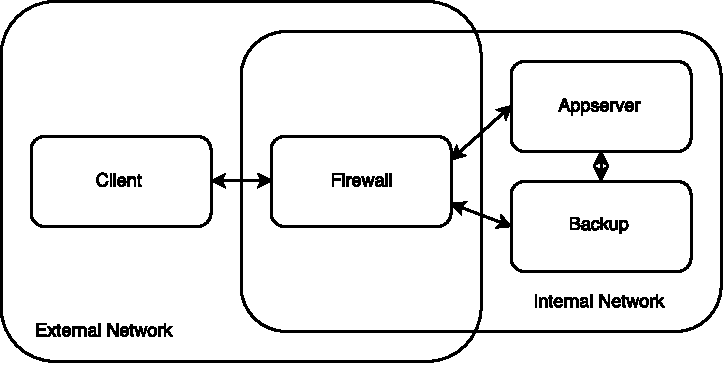
\includegraphics[scale=0.7]{systemoverview.pdf}
	\caption{System overview}
	\label{figure:systemoverview}
\end{figure}

Describe the system's mission,  the system boundaries,
and the overall system architecture, including the main subsystems and
their relationships.   This description should provide a high-level
overview of the system, e.g., suitable for managers, that complements
the more technical description that follows.


\subsection{System Functionality}

Describe the system's functions.


\subsection{Security Design}

Describe the system's security design, including key and session management and 
security of data at rest and in transit.


\subsection{Components}

List all system components and their interfaces, subdivided, for example, into
  categories such as platforms, applications, data records, etc. For
  each component, state its relevant properties.


\ifthenelse{\boolean{showbackdoors}}{
% show for handed-in version

\subsection{Backdoors}

Describe the implemented backdoors. 

\bigskip\noindent
\textbf{Hide this subsection in the version handed over to the reviewing team by setting the flag \texttt{showbackdoors} at the top of this document to \texttt{false}.}


%% do not delete the three lines below
}{ 
% empty for reviewing group's version
} 

\subsection{Additional Material}

You may have additional sections according to your needs.


\section{Risk Analysis and Security Measures}

\subsection{Assets}

\subsubsection{Physical assets}

	\begin{description}
		\item{\textbf{Firewall:}} The firewall is located in a locked and air conditioned room. There is redundant power supply for its server rack. The states of the firewall are running, compromised and down. Running means everything works as expected, compromised means an unauthorized user has had physical access to the machine and down means the firewall is not running.
		\item{\textbf{Application server:}} The application server is located in the same server room with redundant power supply, but in a different rack than the firewall. The same states as in the firewall apply here.
		\item{\textbf{Backup server:}} The backup server is located in the same rack as the application server also equipped with redundant power supply. The same states as in the firewall apply here.
		\item{\textbf{Internal network:}} The internal network is an Ethernet local area network connecting the above mentioned components. The components are connected using layer 2 switches located in the server room. The states are running, compromised and down. A running state indicates that only authorized devices are connected to the network. A compromised state may indicate that an unauthorized user has added his own device to the network and is sniffing connections or injecting and blocking messages. A down state indicates that the network is shut down.
		\item{\textbf{External network:}} The external network connects the firewall to the internet by Ethernet cable using a router that is also located in the server room. The same states as in the internal network apply here.
	\end{description}


\subsubsection{Logical assets}
	\begin{description}
		\item{\textbf{Connectivity:}} Connections between each components and connection to the ISP. For the system to work properly, all components need to be properly connected. The states are connected and not connected.
	\end{description}

\subsubsection{Logical software assets}

	\begin{description}
		\item{\textbf{Firewall operating system:}} The operating system of the firewall is the latest Ubuntu server edition. It is managed by the system administrator who installs all relevant updates and patches within few hours after their release. The states are running, vulnerable, compromised and down. A vulnerable state indicates that the system is not up-to-date and vulnerable to known exploits. A compromised state means the system was already exploited by an attacker.
		\item{\textbf{Firewall service:}} The firewall that separates the internal and external network is the latest edition of the Config Server Firewall (csf). The states are the same as for the Firewall operating system.
		\item{\textbf{Appserver operating system:}} The operating system of the appserver is the same as for the firewall and the same states apply.
		\item{\textbf{Appserver webserver:}} The appserver runs a nginx webserver which handles all http and https requests. It is updated by the system adminstrator. Its states are running, compromised and down. A compromised webserver allows an attacker for example to perform a man-in-the-middle attack.
		\item{\textbf{Appserver application:}} The application is written in python and uses the Django framework. It manages the database and creates, revokes and provides certificates to the user. Both python and the Django framework are regularly updated by the system administrator. The states are similar to the webserver, but in a compromised state, an attacker might change the behaviour of the application.
		\item{\textbf{Appserver certificate authority scripts:}} The functionality as a certificate authority is provided by a set of scripts that rely on the openssl library. The behaviour of the scripts is monitored by the system administrators. The states are the similar to the webserver, but in a compromised state an attacker also has access to certificate related functionality.
		\item{\textbf{Appserver database}} The database is running MySQL and is updated and monitored for misbehaviour by the system administrator. The states are similar to the webserver, but in a compromised state an attacker has altered the database.
		\item{\textbf{Backupserver operating system:}} The operating system of the backupserver is the same as for the firewall and the same states apply.
		\item{\textbf{Backupserver duplicity:}} Duplicity periodically runs on the backupserver and backs up and encrypts valuable data from both the firewall and the appserver such as configurations, logs, certificates, private keys and the database.
	\end{description}

\subsubsection{Logical information assets}
	\begin{description}
		\item{\textbf{User database:}} The database contains user ids, email addresses and hashed passwords. The states are confidential and leaked. A confidential state means that only authorized system administrators and corresponding users have these informations. In a leaked state, an attacker was able to read the whole or part of the database.
		\item{\textbf{Certificates:}} The certificates of each user, the certificate of the webserver and the root certificate. If a certificate is used by someone other than its owner or a certificate is used even though it was revoked, its state is invalid. Otherwise its state is valid. The severity of an invalid certificate depends on which certificate it is and if the usage of such an invalid certificate was detected, since user certificates can easily be revoked.
		\item{\textbf{Appserver configuration:}} Configuration files of different services such as webserver, database, Django, certificate authority or ssh can give insight into how the system behaves and might help detect misconfigured and thus exploitable services. The states are the same as for the user database.
		\item{\textbf{Private keys:}} The private keys for certificates or for ssh connections within the system. Similar states to user database, but the private key is either private or leaked.
		\item{\textbf{Crl:}} The certificate revocation list has to be up-to-date and available to any user. The states are available if any user can get the list and unavailable if this is not the case.
		\item{\textbf{Backupserver configuration:}} Configuration files for services such as duplicity. The states are the same as for appserver configuration.
		\item{\textbf{Logs:}} Logging information about various services. The states are the same as for certificates.
		\item{\textbf{Login credentials:}} Login credentials for ssh connections to different machines that may be leaked by a system administrators and login credentials from users that log into the application server. The states are the same as for the private keys, but for ssh login credential the security concern is much higher.
		\item{\textbf{JWT:}} A JSON web token (JWT) describes an active connection of a user to the webserver. If an attacker manages to compromise the system in a way that he is also part of this connection, the state is compromised. For an active confidential connection the state is confidential and after the connection is closed the state is closed.
		\item{\textbf{Archive key:}} The key that is used to encrypt all backed up data on the backupserver. The states are similar to the private keys.
		\item{\textbf{intermediate \& root key:}} The intermediate key to sign the webserver certificate and user certificates and the root key which signs the intermediate key. The states are similar to private keys.
	\end{description}

\subsubsection{Persons}
\begin{description}
\item{\textbf{User/employee:}} The users of the authenticated mail server, which are employees of iMovie. The state of a user is either loyal or unloyal depending on what relation he has with the company.
\item{\textbf{CA administrator:}} The CA administrators can query the certificate authority for additional information about its state but cannot modify, revoke or create any certificates (except for his own). The states are the same as for User/employee.
  \item{\textbf{System administrator:}} The system administrators manages the system. The states are the same as for User/employee.
  \item{\textbf{Private key holder:}} The CA administrator holds the private key of the root certificate. The states are the same as for User/employee.
\end{description}


\subsubsection{Intangible assets}
\begin{description}
\item{\textbf{User confidence:}} The trust a user has in the system. This is influenced by security breaches, usability of the webserver and other factors. The user either has confidence in the system or not, which means there are two states confident and not confident.
  \end{description}

%software:
%- firewall os
%- firewall service
%- appserver os
%- appserver webserver
%- appserver application
%- appserver ca scripts
%- backupserver os
%- backupserver duplicity

%information:
%database
%- certificates
%- appserver application configuration (webserver, database, django, ca, ssh)
%- private keys
%- crl
%- backupserver application config
%- Logs
%- Login credentials
%- jwt
%- archive key
%- ca key (intermediate \& root key)


%persons:
%- user/employee
%- ca administrator
%- system administrator
%- private key holder

%intangible:
%- user confidence

%Describe the relevant assets and their required security
%  properties. For example, data objects, access restrictions,
%  configurations, etc.

\subsection{Threat Sources}

\begin{description}
\item{\textbf{Nature:}} Environmental factors can hinder the execution of the system. There could be water leaks that would cause damage to servers and lost data.
\item{\textbf{User:}} The employees of iMovie can intentionally misbehave and manipulate the system or unknowingly help an attacker compromise the system.
\item{\textbf{System administrator/Insider:}} A system administrator is a more impactful threat source to the system than a user, since a compromised system administrator leads to much bigger security concerns than a compromised user.
\item{\textbf{Script kiddies:}} Script kiddies most likely do not have iMovie as their primary target, but might still try for example to infect the servers with malware to use them in a botnet. They do not have the skills to infiltrate a well protected system and so the usual security measurements and regular updates should be enough to sufficiently protect against them.
\item{\textbf{Skilled hacker:}} A skilled hacker is a big threat source and the usual security measurements most likely do not give enough protection against such an attacker. He might try to infiltrate the ca server and extract private keys to be able to imitate the webserver itself, issue arbitrary certificates or use the keys to perform man-in-the-middle attacks between employees and extract valuable information. He is most likely to be hired by a competitor or a criminal.
\item{\textbf{Malware:}} There is always the possibility of either directed or undirected malware infection if users with infected systems interact with the system.
\item{\textbf{Organized crime:}} Criminals that try to extract information from the system to blackmail people or steal valuable login credentials that are used across multiple systems.
\item{\textbf{Competitors:}} Competitors that want to undermine the reputation of iMovie, gain knowledge about company secrets or simply cause them damage.
\end{description}

\subsection{Risks Definitions}

%2 points

%Define likelihood, impact and risk level using the following three
%  tables.

%\subsubsection{Tools}

\begin{center}
\begin{table}[h]
\begin{tabularx}{\textwidth}{|l|X|}
\hline
\multicolumn{2}{|c|}{\bf Likelihood} \\
\hline
Likelihood & Description \\
\hline
\hline
High & The threat source is highly motivated and sufficiently capable of exploiting a given vulnerability in order to change the asset’s state. The controls to prevent the vulnerability from being exploited are ineffective.\\
\hline
Medium & The threat source is motivated and capable of exploiting a given vulnerability in order to change the asset’s state, but controls are in place that may impede a successful exploit of the vulnerability. \\
\hline
Low   & The threat source lacks motivation or capabilities to exploit a given vulnerability in order to change the asset’s state. Another possibility that results in a low likelihood is the case where controls are in place that prevent (or at least significantly impede) the vulnerability from being exercised. \\
\hline
\end{tabularx}
\end{table}
\hspace{3em}
\begin{table}[h]
\begin{tabularx}{\textwidth}{|l|X|}
\hline
\multicolumn{2}{|c|}{\bf Impact} \\
\hline
Impact & Description \\
\hline
\hline
High   & The event (1) may result in a highly costly loss of major tangible assets or resources; (2) may significantly violate, harm, or impede an organization’s mission, reputation, or interest; or (3) may result in human death or serious injury. \\
\hline
Medium & The event (1) may result in a costly loss of tangible assets or resources; (2) may violate, harm, or impede an organization’s mission, reputation, or interest, or (3) may result in human injury.\\
\hline
Low & The event (1) may result in a loss of some tangible assets or resources or (2) may noticeably affect an organization’s mission, reputation, or interest.\\
\hline
\end{tabularx}
\end{table}
\end{center}

\vspace{5mm}

\begin{center}
\begin{tabular}{|l|c|c|c|}
\hline
\multicolumn{4}{|c|}{{\bf Risk Level}} \\
\hline
{{\bf Likelihood}} & \multicolumn{3}{c|}{{\bf Impact}} \\ \cline{2-4}
     & Low & Medium & High \\  \hline
 High & Low & Medium & High  \\
\hline
 Medium & Low & Medium & Medium \\
\hline
 Low & Low & Low & Low \\
\hline
\end{tabular}
\end{center}


\subsection{Risk Evaluation}

%7 points

%List all potential threats and the corresponding countermeasures. Estimate the risk based on the information about the threat, the threat sources and the corresponding countermeasure. Adhere to the risk definitions you have given above.

In the following section we will give a risk evaluation for all possible threats and their impact on each of our assets described above. 


\subsubsection{{\it Evaluation physical asset: Hardware}}

%Evaluate the likelihood, impact and the resulting risk,  \emph{after implementation of the corresponding countermeasures}. For each threat, clearly name the threat source and the the threat action.

We can evaluate the risk for our servers and the firewall jointly as the same physical threats apply to them.

\begin{footnotesize}
	\begin{prettytablex}{lXp{3.5cm}lll}
		No. & Threat &  Countermeasure(s) & L & I & Risk \\
		\hline
		1 & Nature: Component failure & Standard configuration, configuration backups, spare machines / components & {\it Medium} & {\it Medium} & {\it Medium} \\
		\hline
		2 & Insider: Accidental or intentional destruction of components & Restrictive room access policies, spare machines / components & {\it Low} & {\it Medium} & {\it Low} \\
		\hline
		3 & Nature: Flooding, fire etc. & Place fire alarm and sprinkler in server room, server room is located in a building on elevated level & {\it Low} & {\it High} & {\it Low} \\
		\hline
		4 & Competitors / Organized crime: Get physical access to server room & Location of server room not public, restrictive access policy & {\it Low} & {\it High} & {\it Low} \\
		\hline
	\end{prettytablex}
\end{footnotesize}

\subsubsection{{\it Evaluation physical asset: Internal network}}

The networking assets include the network cables and the switches/routers used in the server room.

\begin{footnotesize}
	\begin{prettytablex}{lXp{3.5cm}lll}
		No. & Threat &  Countermeasure(s) & L & I & Risk \\
		\hline
		1 & Nature: Component failure & Commodity switch/router, spare cables & {\it Low} & {\it Medium} & {\it Low} \\
		\hline
		2 & Insider: Accidental or intentional destruction of components & Restrictive room access policies, spare cables, backup switch & {\it Low} & {\it Medium} & {\it Low} \\
		\hline
		3 & Insider: Network misconfiguration & Standard configuration, clear documentation & {\it Medium} & {\it Medium} & {\it Medium} \\
		\hline
		4 & Nature: Flooding, fire etc. & Place fire alarm and sprinkler in server room, server room is located in a building on elevated level & {\it Low} & {\it Medium} & {\it Low} \\
		\hline
		5 & Competitors / Organized crime: Get physical access to server room & Location of server room not public, restrictive access policy & {\it Low} & {\it Medium} & {\it Low} \\
		\hline
	\end{prettytablex}
\end{footnotesize}

\subsubsection{{\it Evaluation physical asset: External network}}

\begin{footnotesize}
	\begin{prettytablex}{lXp{3.5cm}lll}
		No. & Threat &  Countermeasure(s) & L & I & Risk \\
		\hline
		1 & Nature: ISP failure & Redundant ISP connection & {\it Low} & {\it Medium} & {\it Low} \\
	\end{prettytablex}
\end{footnotesize}

\subsubsection{{\it Evaluation logical asset: Firewall software}}

\begin{footnotesize}
	\begin{prettytablex}{lXp{3.5cm}lll}
		No. & Threat &  Countermeasure(s) & L & I & Risk \\
		\hline
		1 & System administrator: Mis-configure firewall, purposely include backdoor  &  & {\it Low} & {\it High} & {\it Low} \\
		\hline
		2 & Skilled hacker: Bypass firewall & Use restrictive access rules, regularly update system, keep access logs & {\it Medium} & {\it Medium} & {\it Medium} \\
		\hline
		3 & Espionage / Organized crime: Bypass firewall, use zero day exploits & As above & {\it Medium} & {\it Medium} & {\it Medium} \\
		\hline
	\end{prettytablex}
\end{footnotesize}

\subsubsection{{\it Evaluation logical asset: CA server software}}

\begin{footnotesize}
	\begin{prettytablex}{lXp{3.5cm}lll}
		No. & Threat &  Countermeasure(s) & L & I & Risk \\
		\hline
		1 & System Administrator: Install bad software (e.g. sniffer), do not correctly update/configure system  & Use skilled employees for the task, review system by second party  & {\it Low} & {\it High} & {\it Low} \\
		\hline
		2 & Script kiddies: DDoS & Limit incoming connections from same IP in firewall & {\it Medium} & {\it Medium} & {\it Low} \\
		\hline
		3 & Skilled hacker / Organized Crime: Get system access  & Stop all unused services, close all unnecessary ports  & {\it Low} & {\it High} & {\it Low} \\
		\hline
		4 & Malware: Use server for sending spam or distribute itself on webpages  & Same as above  & {\it HIgh} & {\it Medium} & {\it Medium} \\
		\hline
	\end{prettytablex}
\end{footnotesize}

\subsubsection{{\it Evaluation logical asset: CA server application}}

\begin{footnotesize}
	\begin{prettytablex}{lXp{3.5cm}lll}
		No. & Threat &  Countermeasure(s) & L & I & Risk \\
		\hline
		1 & System Administrator: ?  &  & {\it Low} & {\it High} & {\it Low} \\
		\hline
		2 & Script kiddies / Skilled hacker / Organized Crime: XSS & Validate and sanitize all input  & {\it Low} & {\it High} & {\it Low} \\
		\hline
		3 & Script kiddies / Skilled hacker / Organized Crime: Eavesdrop on communication  & Only use HTTPS for communication & {\it Low} & {\it High} & {\it Low} \\
		\hline
	\end{prettytablex}
\end{footnotesize}

\subsubsection{{\it Evaluation logical asset: CA server database}}

\begin{footnotesize}
	\begin{prettytablex}{lXp{3.5cm}lll}
		No. & Threat &  Countermeasure(s) & L & I & Risk \\
		\hline
		1 & Script kiddies / Skilled hacker / Organized Crime: SQL injection & Sanitize all inputs & {\it Medium} & {\it High} & {\it Medium} \\
		\hline
	\end{prettytablex}
\end{footnotesize}

\subsubsection{{\it Evaluation logical asset: Backup server software}}

\begin{footnotesize}
	\begin{prettytablex}{lXp{3.5cm}lll}
		No. & Threat &  Countermeasure(s) & L & I & Risk \\
		\hline
		1 & System administrator: Turn off backup, misconfigure backup (encryption) & Monitor backup service & {\it Low} & {\it Medium} & {\it Low} \\
		\hline
		2 & Skilled hacker: Get access to system  & Restrict access, turn off unused services, log activities & {\it Low} & {\it High} & {\it Low} \\
		\hline
	\end{prettytablex}
\end{footnotesize}

\subsubsection{{\it Evaluation information asset: User data}}

\begin{footnotesize}
	\begin{prettytablex}{lXp{3.5cm}lll}
		No. & Threat &  Countermeasure(s) & L & I & Risk \\
		\hline
		1 & User: Lose their username and password & Allow them to login using a certificate & {\it Low} & {\it Low} & {\it Low} \\
		\hline
		2 & System Administrator: Intentionally or accidentally modify user data & Don't allow data access to administrators & {\it Low} & {\it Medium} & {\it Low} \\
		\hline
		3 & Script kiddies / Skilled hacker: Steal data & Always use encrypted communication, store data encrypted on backup, restrict access on user data & {\it Medium} & {\it Medium} & {\it Medium} \\
	\end{prettytablex}
\end{footnotesize}

\subsubsection{{\it Evaluation information asset: Certificates}}

\begin{footnotesize}
	\begin{prettytablex}{lXp{3.5cm}lll}
		No. & Threat &  Countermeasure(s) & L & I & Risk \\
		\hline
		1 & User: Lose the certificate & Ability to revoke certificates & {\it Medium} & {\it Low} & {\it Low} \\
		\hline
		2 & System Administrator: Modify data linked to certificate & Restrict data access & {\it Low} & {\it Medium} & {\it Low} \\
		\hline
		3 & Skilled hacker: Issue bogus certificate & Don't allow user registration, log certificate creations & {\it Low} & {\it High} & {\it Low} \\
		\hline
	\end{prettytablex}
\end{footnotesize}

\subsubsection{{\it Evaluation information asset: Private keys}}

\begin{footnotesize}
	\begin{prettytablex}{lXp{3.5cm}lll}
		No. & Threat &  Countermeasure(s) & L & I & Risk \\
		\hline
		1 & System Administrator: Leak to external party & Only root is allowed to access private keys & {\it Low} & {\it High} & {\it Low} \\
		\hline
		2 & Script kiddies / Skilled hacker: Steal private keys & Private keys are only accessible for root users, keys are encrypted in transfer & {\it Low} & {\it High} & {\it Low} \\
		\hline
	\end{prettytablex}
\end{footnotesize}

\subsubsection{{\it Evaluation information asset: CRL}}

\begin{footnotesize}
	\begin{prettytablex}{lXp{3.5cm}lll}
		No. & Threat &  Countermeasure(s) & L & I & Risk \\
		\hline
		1 & System Administrator: Insert fake or remove real entries & Access write rights to root & {\it Low} & {\it High} & {\it Low} \\
		\hline
		2 & Script kiddies / Skilled hacker: Same as for the sysadmin & Same as in 1 & {\it Low} & {\it High} & {\it Low} \\
		\hline
	\end{prettytablex}
\end{footnotesize}

\subsubsection{{\it Evaluation information asset: Server configuration}}

\begin{footnotesize}
	\begin{prettytablex}{lXp{3.5cm}lll}
		No. & Threat &  Countermeasure(s) & L & I & Risk \\
		\hline
		1 & System Administrator: Leak configuration & Place configuration in standard place (secured by access policies) & {\it Low} & {\it Medium} & {\it Low} \\
		\hline
		2 & Script kiddies / Skilled hacker: Alter configuration (e.g. weaken preferred security algorithms) & As above, additionally backup config incrementally (spot alterations) & {\it Low} & {\it High} & {\it Low} \\
		\hline
		3 & Malware: Delete or alter configuration randomly & Backup configuration (incremental), access logs, restrictive access policies & {\it Medium} & {\it High} & {\it Medium} \\
		\hline
		4 & Competitors / Espionage: Access configuration and use for own system  &  & {\it Low} & {\it Medium} & {\it Low} \\
		\hline
	\end{prettytablex}
\end{footnotesize}

\subsubsection{{\it Evaluation information asset: Logs}}

\begin{footnotesize}
	\begin{prettytablex}{lXp{3.5cm}lll}
		No. & Threat &  Countermeasure(s) & L & I & Risk \\
		\hline
		1 & System Administrator: Accidentally or intentionally delete logs & Policy to not delete logs before they are backed up & {\it Low} & {\it Medium} & {\it Low} \\
		\hline
		2 & Script kiddies / Skilled hacker: Insert or delete messages from the logs & Restrict access to logs to application and root & {\it Medium} & {\it Medium} & {\it Medium} \\
		\hline
		3 & Malware: Insert random logs & Restrict access to logs to application and root & {\it Low} & {\it Medium} & {\it Low} \\
		\hline
	\end{prettytablex}
\end{footnotesize}

\subsubsection{{\it Evaluation information asset: Login credentials}}

\begin{footnotesize}
	\begin{prettytablex}{lXp{3.5cm}lll}
		No. & Threat &  Countermeasure(s) & L & I & Risk \\
		\hline
		1 & System Administrator: Forget login credentials & Backup offline, allow login with ssh key & {\it Medium} & {\it High} & {\it Low} \\
		\hline
		2 & Script kiddies / Skilled hacker: Brute force password guessing & Restrict amount of connections from same IP, enforce strong passwords & {\it Low} & {\it High} & {\it Low} \\
		\hline
	\end{prettytablex}
\end{footnotesize}

\subsubsection{{\it Evaluation information asset: JWT}}

\begin{footnotesize}
	\begin{prettytablex}{lXp{3.5cm}lll}
		No. & Threat &  Countermeasure(s) & L & I & Risk \\
		\hline
		1 & User: Lose JWT & Saved in browser session & {\it Low} & {\it Low} & {\it Low} \\
		\hline
		3 & Script kiddies: Steal JWT from a not closed browser window & Short lifetime of token & {\it Low} & {\it High} & {\it Low} \\
		\hline
		4 & Skilled hacker: Steal JWT (e.g. by malicious browser plugin) & Only store JWT in local session, short lifetime of token, enforce PW/certificate login afterwards & {\it Low} & {\it High} & {\it Low} \\
		\hline
	\end{prettytablex}
\end{footnotesize}

\subsubsection{{\it Evaluation information asset: Archive key}}

\begin{footnotesize}
	\begin{prettytablex}{lXp{3.5cm}lll}
		No. & Threat &  Countermeasure(s) & L & I & Risk \\
		\hline
		1 & System Administrator: Lose key (stored offline) & Store at different locations (e.g. in several safes) & {\it Low} & {\it High} & {\it Low} \\
		\hline
	\end{prettytablex}
\end{footnotesize}

\subsubsection{{\it Evaluation information asset: Root key}}

\begin{footnotesize}
	\begin{prettytablex}{lXp{3.5cm}lll}
		No. & Threat &  Countermeasure(s) & L & I & Risk \\
		\hline
		2 & System Administrator: Lose key (stored offline) & Store at different locations (e.g. in several safes) & {\it Low} & {\it High} & {\it Low} \\
		\hline
	\end{prettytablex}
\end{footnotesize}

\subsubsection{{\it Evaluation person asset: User/employee}}

\subsubsection{{\it Evaluation person asset: CA administrator / insider}}

\subsubsection{{\it Evaluation person asset: System administrator}}

\subsubsection{{\it Evaluation person asset: Private key holder}}

\subsubsection{{\it Evaluation intangible asset: User confidence}}


\subsubsection{Detailed Description of Selected Countermeasures}

Optionally explain the details of the countermeasures mentioned above.



\subsubsection{Risk Acceptance}

List all medium and high risks, according to the evaluation above. For each risk, propose additional countermeasures that could be implemented to further reduce the risks.

\begin{footnotesize}
\begin{prettytablex}{p{2cm}X}
No. of threat & Proposed additional countermeasure including expected impact  \\
\hline
... & ... \\
\hline
... & ... \\
\hline
\end{prettytablex}
\end{footnotesize}

\end{document}

%%% Local Variables: 
%%% mode: latex
%%% TeX-master: "../../book"
%%% End: 
